% Options here are passed to the article class.
% Most common options: 10pt, 11pt, 12pt
\documentclass[10pt]{datasheet}

% Input encoding and typographical rules for English language
\usepackage[utf8]{inputenc}
\usepackage[english]{babel}
\usepackage[english]{isodate}

% tikz is used to draw images in this example, but you can
% also use \includegraphics{}.
\usepackage{graphicx}
\usepackage{float}
\usepackage{subcaption}

% These define global texts that are used in headers and titles.
\title{EC07: Unstackable Item Encoder}
\author{Basil, Pyra, 77}
\tags{encoders, unstackable}
\date{25 December 2024}
\revision{Revision 1}
\begin{document}
\maketitle

\section{Features}

\begin{itemize}
\item{Uses Pyra's unstackable sorter to sort items at hopperspeed.}
\item{Built-in box loaders for each item type.}
\item{Sorts music discs, enchanted books, potions, flint \& steel, shears, powdered snow buckets, lava buckets, water buckets, boats, armor and minecarts in that order.}
\item{Fully hopperlocked.}
\item{Built-in queue for output.}
\end{itemize}

\section{Applications}

\begin{itemize}
\item{Sorting and encoding unstackable items.}
\end{itemize}

\section{General Description}
The EC07 Unstackable Item Encoder is a device that sorts unstackable items using Pyra's unstackable sorter and then outputs boxes of the sorted items along with an encoded signal. The device features a built-in queue to output boxes of items upon request. The device is fully hopperlocked and is designed to sort music discs, enchanted books, potions, flint \& steel, shears, powdered snow buckets, lava buckets, water buckets, boats, armor and minecarts in that order. Item codes can be set by modifying the read-only memory of the device. See the corresponding \href{https://www.youtube.com/watch?v=1yDuKrriiYI}{explanation video on Youtube}.
\vfill\break

\begin{figure}[H]
    \centering
    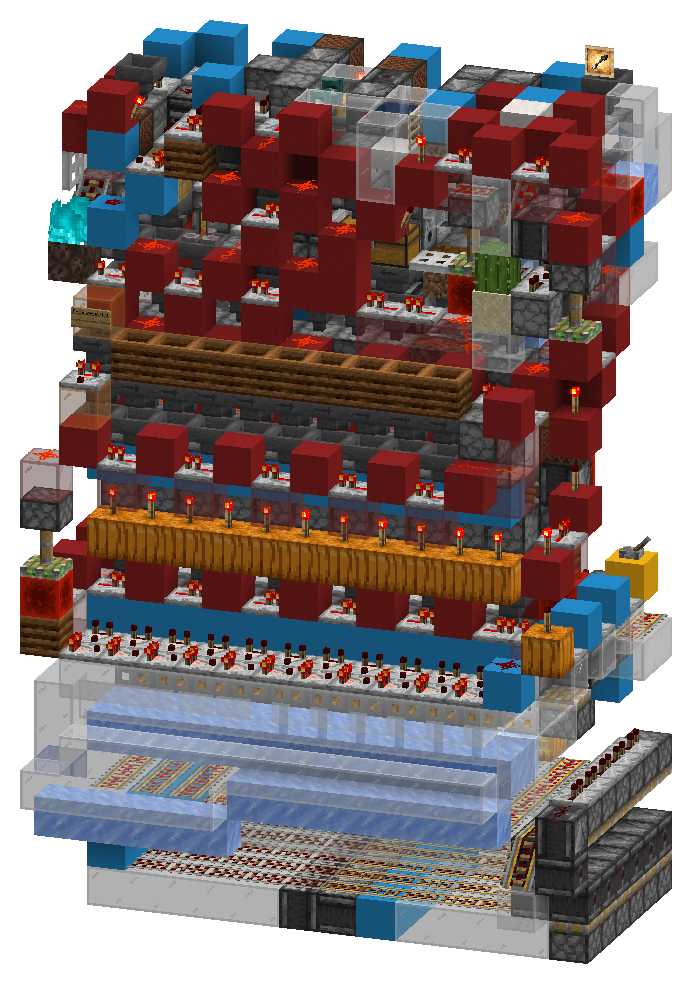
\includegraphics[width=0.48\textwidth]{area_render_33_.png}
    \caption{\centering Unstackable Item Encoder}
\end{figure}

% For wide tables, a single column layout is better. It can be switched
% page-by-page.
\onecolumn

\begin{figure}[H]
    \centering
    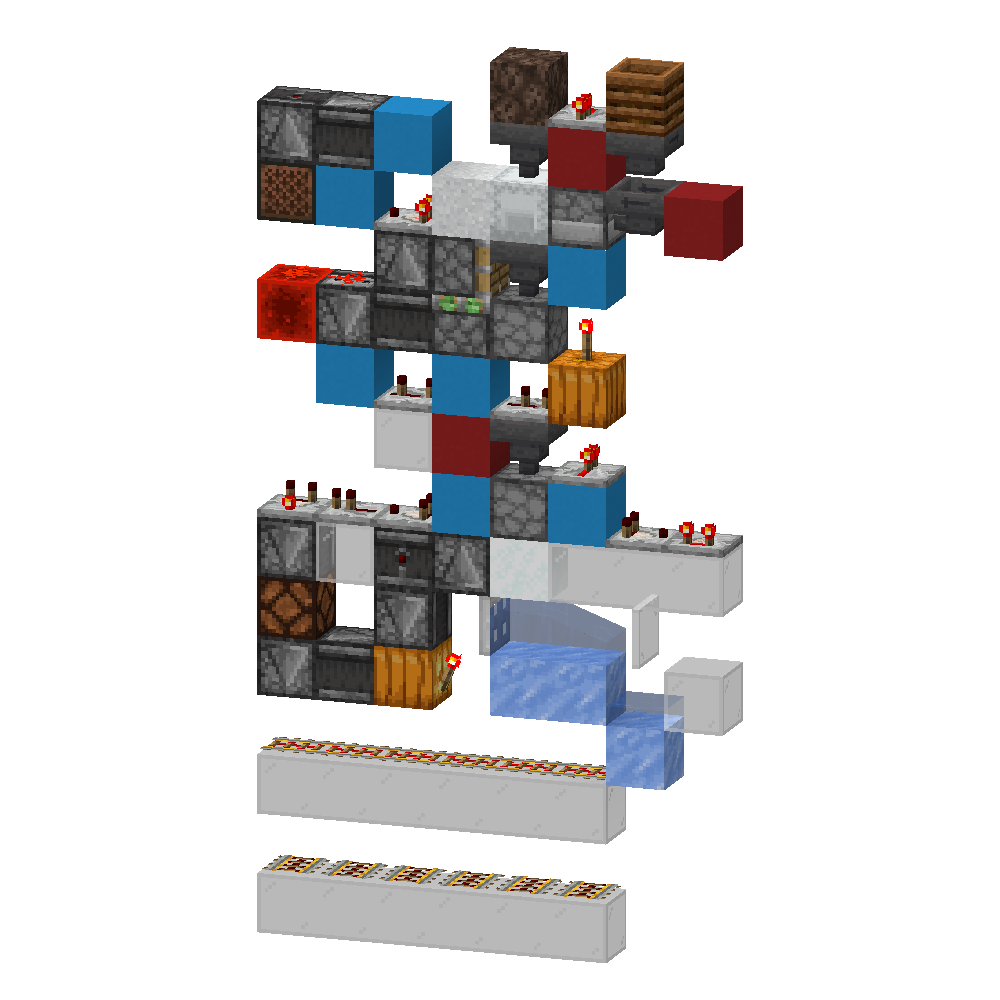
\includegraphics[width=0.6\textwidth]{slice.png}
    \caption{\centering Slice of Unstackable Item Encoder Output Controller}
\end{figure}

\section{Configuring Item Codes}
Item codes can be set by replacing the white stained glass blocks at the bottom of the device with observers corresponding to the desired item code. No codes are set by default.

\begin{figure}[H]
    \centering
    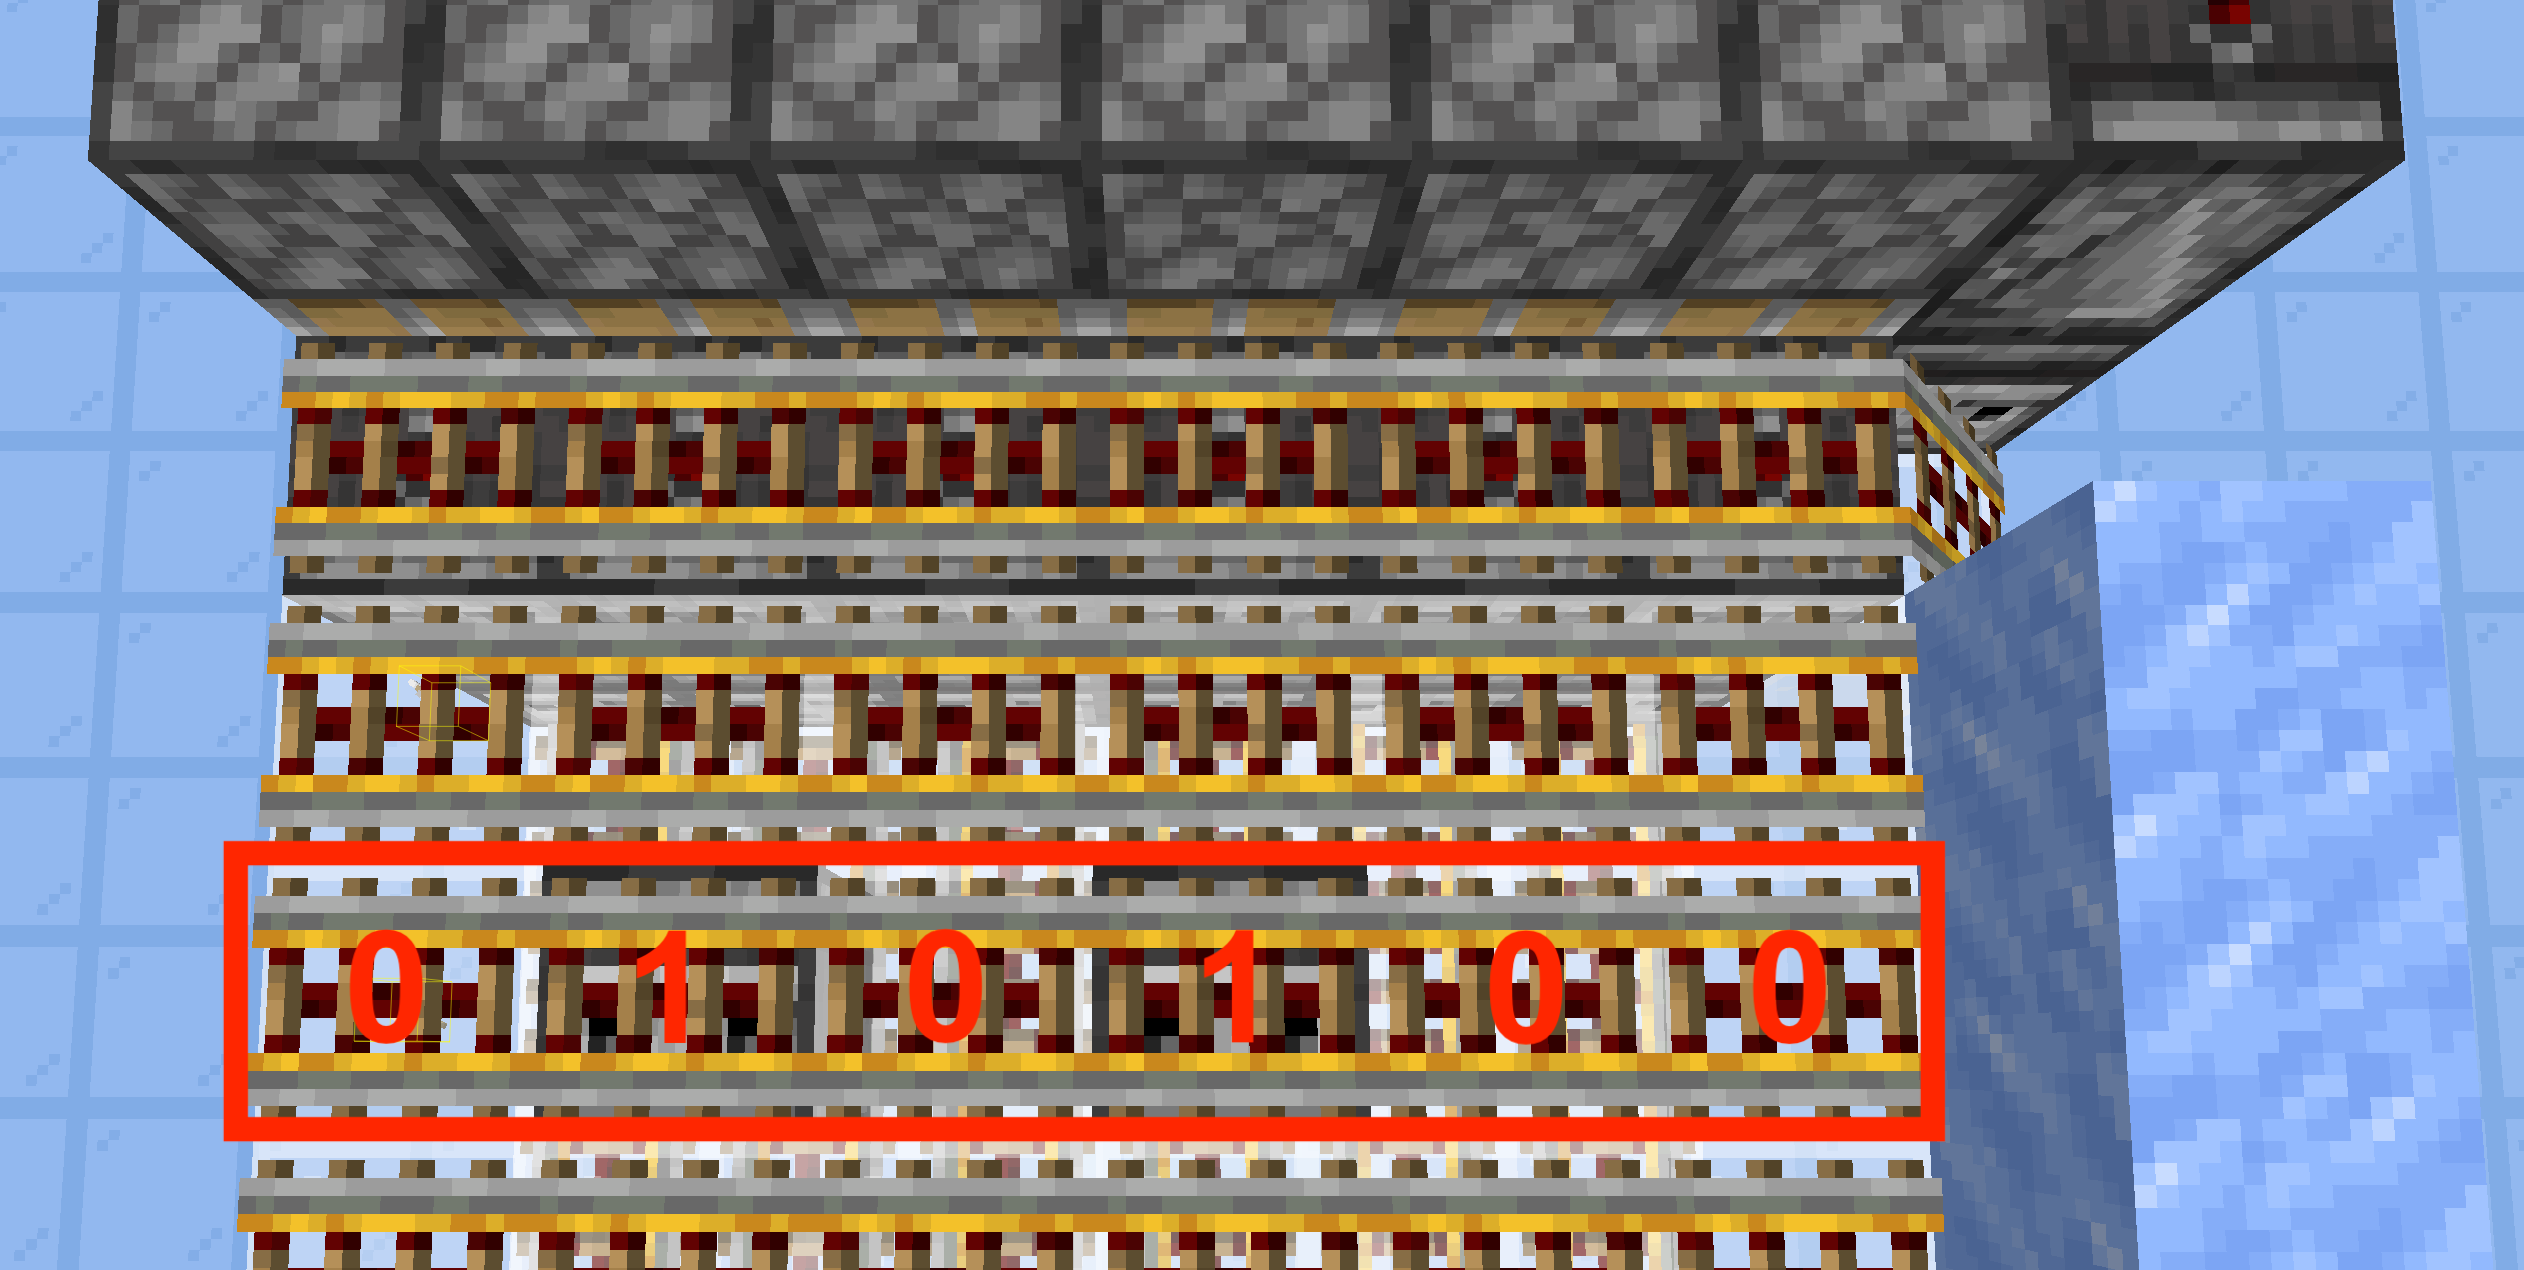
\includegraphics[width=0.48\textwidth]{setting.png}
    \caption{\centering Setting Item Codes}
\end{figure}

\newpage
\section{Device Specifications}

\begin{table}[H]
    \caption{Inputs}
    \begin{tabularx}{\textwidth}{l | c | X}
        \thickhline
        \textbf{Name} & \textbf{Range} & \textbf{Description} \\
        \hline
        Unstackable input & Item & Unstackable items to be sorted. Barrel input. \\
        \hline
        Arrows & Item & Arrow items to break armor. Barrel input. \\
        \hline
        Request & Pulse & Request for output. Noteblock input. \\
        \hline
        Hopperlocking & 0-1 & Controls hopperlocking. Lever input. \\
        \thickhline
\end{tabularx}
\end{table}

\begin{table}[H]
    \caption{Outputs}
    \begin{tabularx}{\textwidth}{l | c | X}
        \thickhline
        \textbf{Name} & \textbf{Range} & \textbf{Description} \\
        \hline
        Box output & Box & Box of sorted items output on request. Waterstream output. \\
        \hline
        Item code & Code & 6 bit encoded signal corresponding to item type of output. \\
        \thickhline
\end{tabularx}
\end{table}

\begin{table}[H]
    \caption{Device Specifications}
    \begin{tabularx}{\textwidth}{l | c c c | c | X}
        \thickhline
        \textbf{Parameter} & \textbf{Min.} & \textbf{Typ.} & \textbf{Max.} &
        \textbf{Unit} & \textbf{Conditions} \\
        \hline
        Throughput  & 8 & - & - & gt & Item input \\
        \hline
        MC Version & 1.21 & 1.21.4 & - & MCV & Latest version at time of writing: 1.21.4\\
        \hline
        Dimensions & & 8 x 22 x 14 & & Blocks & \\
        \thickhline
\end{tabularx}
\end{table}
\section{Testing Data}
\begin{table}[H]
\caption{Executed Tests}
\begin{tabularx}{\textwidth}{l | X}
    \thickhline
    \textbf{Test} & \textbf{Result} \\
    \hline
    Throughput test & Device was able to function with various unstackable input \\
    \hline
    Output test & Device was able to output boxes with item codes \\
    \thickhline
\end{tabularx}
\end{table}

\section{Download Information}
\begin{table}[H]
    \caption{Download Information}
    \begin{tabularx}{\textwidth}{l | l | l | X}
        \thickhline
        \textbf{Identifier} & \textbf{MC} & \textbf{File} & \textbf{Description} \\
        \hline
        EC07 & 1.21 & \href{https://github.com/Soontech-Annals/Archive/blob/2b73adfd252c5e2cf9d202454dbef78a586bc482/Archive/encoders/EC07\%20Unstackable\%20Item\%20Encoder/EC07\_Unstackable\_Item\_Encoder.litematic?raw=1}{EC07\_Unstackable\_Item\_Encoder.litematic} & Schematic of device. \\
        \hline
        \thickhline
    \end{tabularx}
\end{table}

\end{document}

